\documentclass[11pt]{article}

\usepackage[margin=1in]{geometry}
\usepackage{times}
\usepackage{graphicx}
\usepackage{booktabs}
\usepackage{amsmath,amssymb,amsthm}
\usepackage{hyperref}
\usepackage{natbib}
\usepackage{microtype}
\usepackage{caption}
\usepackage{url}
\usepackage{enumitem}
\usepackage{array}

\hypersetup{colorlinks=true,linkcolor=black,citecolor=blue,urlcolor=blue}
\captionsetup{
  font=small,
  labelfont=bf,
  skip=6pt,
  justification=centering,
  singlelinecheck=true
}
\setlist[itemize]{leftmargin=1.2em,itemsep=2pt,topsep=3pt,parsep=0pt}
\setlength{\parskip}{0.3em}
\setlength{\parindent}{1.15em}
\setlength{\tabcolsep}{10pt}
\renewcommand{\arraystretch}{1.12}

% Keep caption + body together; never stretch columns.
\newcommand{\ctable}[3]{%
  \par\medskip\noindent
  \begin{minipage}{\linewidth}
    \centering
    \captionof{table}{#1}\label{#2}
    \vspace{0.4em}
    #3
  \end{minipage}
  \par\medskip}
\newcommand{\cfigure}[3]{%
  \par\medskip\noindent
  \begin{minipage}{\linewidth}
    \centering
    #3
    \vspace{0.35em}
    \captionof{figure}{#1}\label{#2}
  \end{minipage}
  \par\medskip}

\newtheorem{hypothesis}{Hypothesis}
\newtheorem{researchquestion}{RQ}

\title{Shared Priors, Not Assistance in General:\\
What Public Co-Writing Data Support about Homogenization}

\author{
Babandeep Singh\\
\texttt{babandeep193@gmail.com}\\
Independent Researcher
}

\date{Technical Report / Workshop Note\\[0.25em]\today}

\begin{document}
\maketitle

\begin{abstract}
This short technical report separates two often-joined worries about language-model writing help: homogenization of outputs, and later transfer debt.
We ask only what four public corpora can support.
Re-analyzing those releases, we find one narrow positive result and several negative or non-identified ones.
In the Padmakumar and He co-writing essays, InstructGPT reduces within-topic diversity relative to solo writing and relative to GPT-3; model spans under InstructGPT are less diverse than user spans.
Topic-level permutation tests reject the null for both InstructGPT contrasts ($p=0.002$ and $p=0.002$), while the solo-versus-GPT-3 contrast does not ($p=0.72$).
The solo--InstructGPT bootstrap interval is wide and includes zero, so that contrast is suggestive rather than definitive.
Vectorizer robustness checks preserve the same ordering.
CoAuthor shows no strong acceptance dose-response on group diversity.
Moon et al.\ materials show a concentrated model prior, but not a clean post-ChatGPT lexical collapse.
Public study-companion logs cannot identify transfer debt.
We keep prior-driven homogenization as a limited claim, drop assistance-as-such claims, and leave debt open.
\end{abstract}

\noindent\textbf{Note type:} workshop-style technical report (public-data reanalysis; no new human experiment).

\noindent\textbf{Keywords:} large language models, homogenization, shared priors, co-writing, open reanalysis

\section{Introduction}

Language models improve local drafting.
They also create a population question.
If many writers condition on one generative prior, the set of answers across people can shrink even while each person feels faster~\citep{padmakumar2024diversity,anderson2024homogenization,acemoglu2026collapse}.
A second question is cognitive debt: weaker performance once the helper is removed~\citep{kosmyna2025eeg,barcaui2025crutch,risko2016offloading,parasuraman1997automation}.

These worries are often told as one mechanism, \emph{cognitive convergence}: offloading onto a shared prior that both compresses diversity and leaves a transfer cost.
That framing is a research program, not a finding, until public data can carry it.

This note is a falsification-oriented reassessment of four public corpora, written as a short workshop-style technical report rather than a full conference paper.
We rank claims by support:
\begin{itemize}
  \item \textbf{Keep:} shared feedback-tuned priors can compress co-written diversity.
  \item \textbf{Drop:} any LM assistance homogenizes.
  \item \textbf{Leave open:} transfer debt as part of the same mechanism.
\end{itemize}

\paragraph{What this note does.}
(1)~Reanalyzes Padmakumar and He~\citep{padmakumar2024diversity} with topic bootstrap intervals, permutation tests, and vectorizer robustness.
(2)~Checks CoAuthor for an acceptance dose pattern on group diversity~\citep{lee2022coauthor}.
(3)~Contrasts a concentrated model prior with mixed observational era effects in Moon et al.~\citep{moon2026disjunction,osfyd94z2026}.
(4)~States an explicit non-identification result for debt in public study-companion logs~\citep{simsek2025companion,osfswytk2025}.

\section{Related Work}

Padmakumar and He~\citep{padmakumar2024diversity} provide the cleanest public writing contrast: solo, GPT-3, and InstructGPT essays with authorship masks, separating feedback-tuned help from base-model help.
Anderson et al.~\citep{anderson2024homogenization} report ideation homogenization without public microdata.
Moon et al.~\citep{moon2026disjunction,osfyd94z2026} release admissions-writing materials that separate surface diversity from conceptual originality and include matched human--model and within-subject GPT conditions.
Acemoglu et al.~\citep{acemoglu2026collapse} formalize population knowledge collapse when many agents share similar AI outputs.

Lee et al.~\citep{lee2022coauthor} release CoAuthor, a large GPT-3 co-writing log with suggestion accepts but no unaided arm.
Dell'Acqua et al.~\citep{dellacqua2025frontier} show AI can raise or hurt task performance depending on the task; that jagged frontier is about quality, not cross-person diversity.

Cognitive offloading~\citep{risko2016offloading} and automation misuse~\citep{parasuraman1997automation} predate LLMs.
Kosmyna et al.~\citep{kosmyna2025eeg}, Barcaui~\citep{barcaui2025crutch}, and Lee et al.~\citep{lee2025critical} report debt, retention cost, or effort and confidence shifts, mostly without open microdata for reanalysis.
{\c{S}}im{\c{s}}ek et al.~\citep{simsek2025companion,osfswytk2025} release companion logs, but both processed arms still use ChatGPT, so debt versus unaided learning is not identified.

This note does not propose a new theory.
It ranks what the public corpora above can already support.

\section{Claims}

\begin{hypothesis}[H1]
Within-topic diversity is lower for InstructGPT essays than for solo essays.
\end{hypothesis}
\begin{hypothesis}[H2]
Within-topic diversity is lower for InstructGPT than for GPT-3.
\end{hypothesis}
\begin{hypothesis}[H3]
Under InstructGPT, model spans are less diverse than user spans.
\end{hypothesis}

\begin{researchquestion}[RQ1]
In CoAuthor, does higher suggestion acceptance reduce cross-session diversity?
\end{researchquestion}
\begin{researchquestion}[RQ2]
In Moon et al.\ materials, is the model prior narrower than unaided human writing, and do observational post-ChatGPT essays show lower diversity?
\end{researchquestion}
\begin{researchquestion}[RQ3]
Can public study-companion logs identify transfer debt versus unaided learning?
\end{researchquestion}

\section{Method}

\subsection{Data}
\textbf{Padmakumar and He}~\citep{padmakumar2024diversity}: after dropping essays under 40 words, solo $N=99$, GPT-3 $N=97$, InstructGPT $N=100$, across ten topics.
User and model texts use authorship labels \texttt{U} and \texttt{A}.

\textbf{CoAuthor}~\citep{lee2022coauthor}: final documents with at least 40 words ($N=1218$); acceptance rate among sessions with at least one suggestion request ($N=1185$).

\textbf{Moon et al.}~\citep{moon2026disjunction,osfyd94z2026}: released pre/post aggregates, matched within-prompt distances, and within-subject unaided / GPT-revised / GPT-generated essays ($N=203$ per condition).

\textbf{{\c{S}}im{\c{s}}ek et al.}~\citep{simsek2025companion,osfswytk2025}: processed scores for summary versus transcript ($N=101$) and summary versus question ($N=215$).

\subsection{Measures}
Primary diversity for Padmakumar and CoAuthor is one minus mean pairwise TF--IDF cosine similarity within a stratum (topic or acceptance tercile), with a vectorizer fit on the relevant corpus.
Padmakumar also reports MiniLM embedding diversity.
Homogenization versus solo is $H=(D_{\mathrm{solo}}-D)/D_{\mathrm{solo}}$.
For Moon materials we use released word and document distances.
For learning logs we compare transfer by condition and help-count correlations within arm.

\subsection{Inference for Study 1}
We treat topics as the resampling unit.
For each condition we compute within-topic diversity, then draw $5000$ topic bootstraps to form $95\%$ intervals for mean $D$ and for pairwise gaps.
We also run one-sided essay-label permutation tests within topics ($999$ permutations): under the null, solo and InstructGPT essays are exchangeable within topic.
Robustness checks recompute the three condition means with unigram TF--IDF and with stop-words retained.
Analysis code: \texttt{scripts/study1\_stats.py}.

\section{Results}

\subsection{Study 1: the claim that holds}
Within-topic TF--IDF diversity is $0.780$ (solo), $0.788$ (GPT-3), and $0.740$ (InstructGPT), so $H=0.051$ for InstructGPT versus solo (Table~\ref{tab:study1}).
Embedding diversity falls from $0.359$ to $0.329$ (GPT-3) and $0.298$ (InstructGPT).

\ctable{Study 1 main estimates (Padmakumar and He).}{tab:study1}{%
\small
\begin{tabular}{@{}lrrrr@{}}
\toprule
Condition & $N$ & TF--IDF $D$ & Emb.\ $D$ & $H$ \\
\midrule
solo & 99 & 0.780 & 0.359 & \phantom{-}0.000 \\
gpt3 & 97 & 0.788 & 0.329 & $-0.010$ \\
instructgpt & 100 & 0.740 & 0.298 & \phantom{-}0.051 \\
\bottomrule
\end{tabular}}

Table~\ref{tab:contrasts} reports topic-bootstrap gaps.
The GPT-3 minus InstructGPT gap is $0.047$ (95\% CI $[0.001, 0.097]$; permutation $p=0.002$).
The solo minus InstructGPT gap is $0.040$ (CI $[-0.018, 0.099]$; $p=0.002$); $90.7\%$ of bootstrap replicates are positive.
The solo minus GPT-3 gap is near zero ($p=0.72$).
H1 and H2 are directionally consistent with the permutation tests and with the GPT-3 contrast interval; the solo--InstructGPT bootstrap interval includes zero, so we treat H1 as limited support rather than a definitive estimate.
InstructGPT is below solo in $60\%$ of topics and below GPT-3 in $80\%$.

\ctable{Study 1 diversity gaps (topic bootstrap $95\%$ CIs; one-sided permutation $p$).}{tab:contrasts}{%
\small
\setlength{\tabcolsep}{5pt}
\begin{tabular}{@{}lrrrr@{}}
\toprule
Contrast & Est. & CI lo & CI hi & $p$ \\
\midrule
solo $-$ IGPT & \phantom{-}0.040 & $-0.018$ & 0.099 & 0.002 \\
GPT-3 $-$ IGPT & \phantom{-}0.047 & \phantom{-}0.001 & 0.097 & 0.002 \\
solo $-$ GPT-3 & $-0.008$ & $-0.063$ & 0.046 & 0.725 \\
\bottomrule
\end{tabular}}

Under InstructGPT, model spans are less diverse than user spans (Table~\ref{tab:auth}: TF--IDF $0.820$ vs $0.835$; embeddings $0.316$ vs $0.364$).
Under GPT-3, model spans are more diverse than user spans.
H3 is directional; the InstructGPT authorship gap is small and its topic-bootstrap interval includes zero.

\ctable{Authorship split (within-topic diversity).}{tab:auth}{%
\small
\begin{tabular}{@{}lrrr@{}}
\toprule
Condition & $N$ & TF--IDF $D$ & Emb.\ $D$ \\
\midrule
gpt3 user & 96 & 0.849 & 0.361 \\
gpt3 model & 94 & 0.897 & 0.453 \\
instructgpt user & 98 & 0.835 & 0.364 \\
instructgpt model & 98 & 0.820 & 0.316 \\
\bottomrule
\end{tabular}}

\paragraph{Robustness.}
Unigram TF--IDF and stop-word retention preserve the same order: InstructGPT $<$ solo $\approx$ GPT-3 (Table~\ref{tab:rob}).

\ctable{Vectorizer robustness (mean within-topic $D$).}{tab:rob}{%
\small
\begin{tabular}{@{}lrrr@{}}
\toprule
Spec & solo & gpt3 & instructgpt \\
\midrule
main (1--2 gram) & 0.780 & 0.788 & 0.740 \\
unigram & 0.743 & 0.748 & 0.700 \\
no stop-word filter & 0.726 & 0.730 & 0.692 \\
\bottomrule
\end{tabular}}

\subsection{Study 2: the dose pattern that does not}
In CoAuthor, group diversity is almost flat across acceptance terciles: $0.929$, $0.929$, and $0.922$ (Table~\ref{tab:coauthor}).
Acceptance correlates only mildly with similarity to the corpus centroid ($\rho=+0.178$).
Never-request sessions are rare ($N=33$) and are not a clean solo control.
RQ1: weak atypicality signal, no strong group-diversity dose curve.

\ctable{CoAuthor by acceptance tercile.}{tab:coauthor}{%
\small
\begin{tabular}{@{}lrrr@{}}
\toprule
Bin & $N$ & Accept rate & TF--IDF $D$ \\
\midrule
low & 395 & 0.427 & 0.929 \\
mid & 395 & 0.731 & 0.929 \\
high & 395 & 0.930 & 0.922 \\
\bottomrule
\end{tabular}}

\subsection{Study 3: a narrow model prior, mixed era effects}
Matched within-prompt document distance is $0.302$ for human essays versus $0.116$ for GPT essays.
Within subjects, document distance falls from $0.293$ (unaided) to $0.219$ (GPT-revised) and $0.178$ (GPT-generated); $92\%$--$95\%$ of people are lower under GPT than under their own unaided essay (Table~\ref{tab:moon}).

\ctable{Moon et al.\ distance summaries.}{tab:moon}{%
\small
\begin{tabular}{@{}llrr@{}}
\toprule
Panel & Condition & $N$ & Doc.\ distance \\
\midrule
Matched & human & n/a & 0.302 \\
Matched & gpt & n/a & 0.116 \\
\midrule
Within & unaided & 203 & 0.293 \\
Within & gpt revised & 203 & 0.219 \\
Within & gpt generated & 203 & 0.178 \\
\bottomrule
\end{tabular}}

Observational era contrasts are mixed.
Word distance is slightly higher after ChatGPT ($0.832$ vs $0.830$), while document distance is slightly lower ($0.214$ vs $0.222$).
These are calendar labels, not individual AI-use labels.
RQ2: model prior narrowing is supported; population lexical collapse is not.

\subsection{Study 4: debt is not identified here}
Both arms in each {\c{S}}im{\c{s}}ek et al.\ study use ChatGPT~\citep{simsek2025companion}.
Transfer means differ by roughly $0.1$--$0.2$ points across arms; help-count correlations with transfer are near zero.
RQ3: not testable as debt versus unaided learning.
Debt estimates in Kosmyna et al.~\citep{kosmyna2025eeg} and Barcaui~\citep{barcaui2025crutch} remain external.

\subsection{Claim map}
Table~\ref{tab:verdicts} and Figure~\ref{fig:multi} summarize the four-corpus evidence.

\ctable{What public microdata support.}{tab:verdicts}{%
\small
\begin{tabular}{@{}p{0.50\linewidth}ll@{}}
\toprule
Claim & Verdict & Where \\
\midrule
InstructGPT homogenizes vs solo/GPT-3 & Limited support & Padmakumar \\
Any LM assistance homogenizes & Not supported & Padmakumar \\
Accept dose on group diversity & Weak / mixed & CoAuthor \\
Model-only text narrower than human & Supported & Moon et al. \\
Post-ChatGPT word-diversity collapse & Not supported & Moon et al. \\
Transfer debt in public learning logs & Not testable & {\c{S}}im{\c{s}}ek et al. \\
Unified cognitive convergence & Not established & All \\
\bottomrule
\end{tabular}}

\cfigure{Evidence map across corpora.
(A)~InstructGPT lowers diversity; GPT-3 does not.
(B)~Under InstructGPT, model spans are the less diverse component.
(C)~CoAuthor acceptance barely moves group diversity.
(D)~GPT-generated and GPT-revised essays are narrower than unaided essays.}{fig:multi}{%
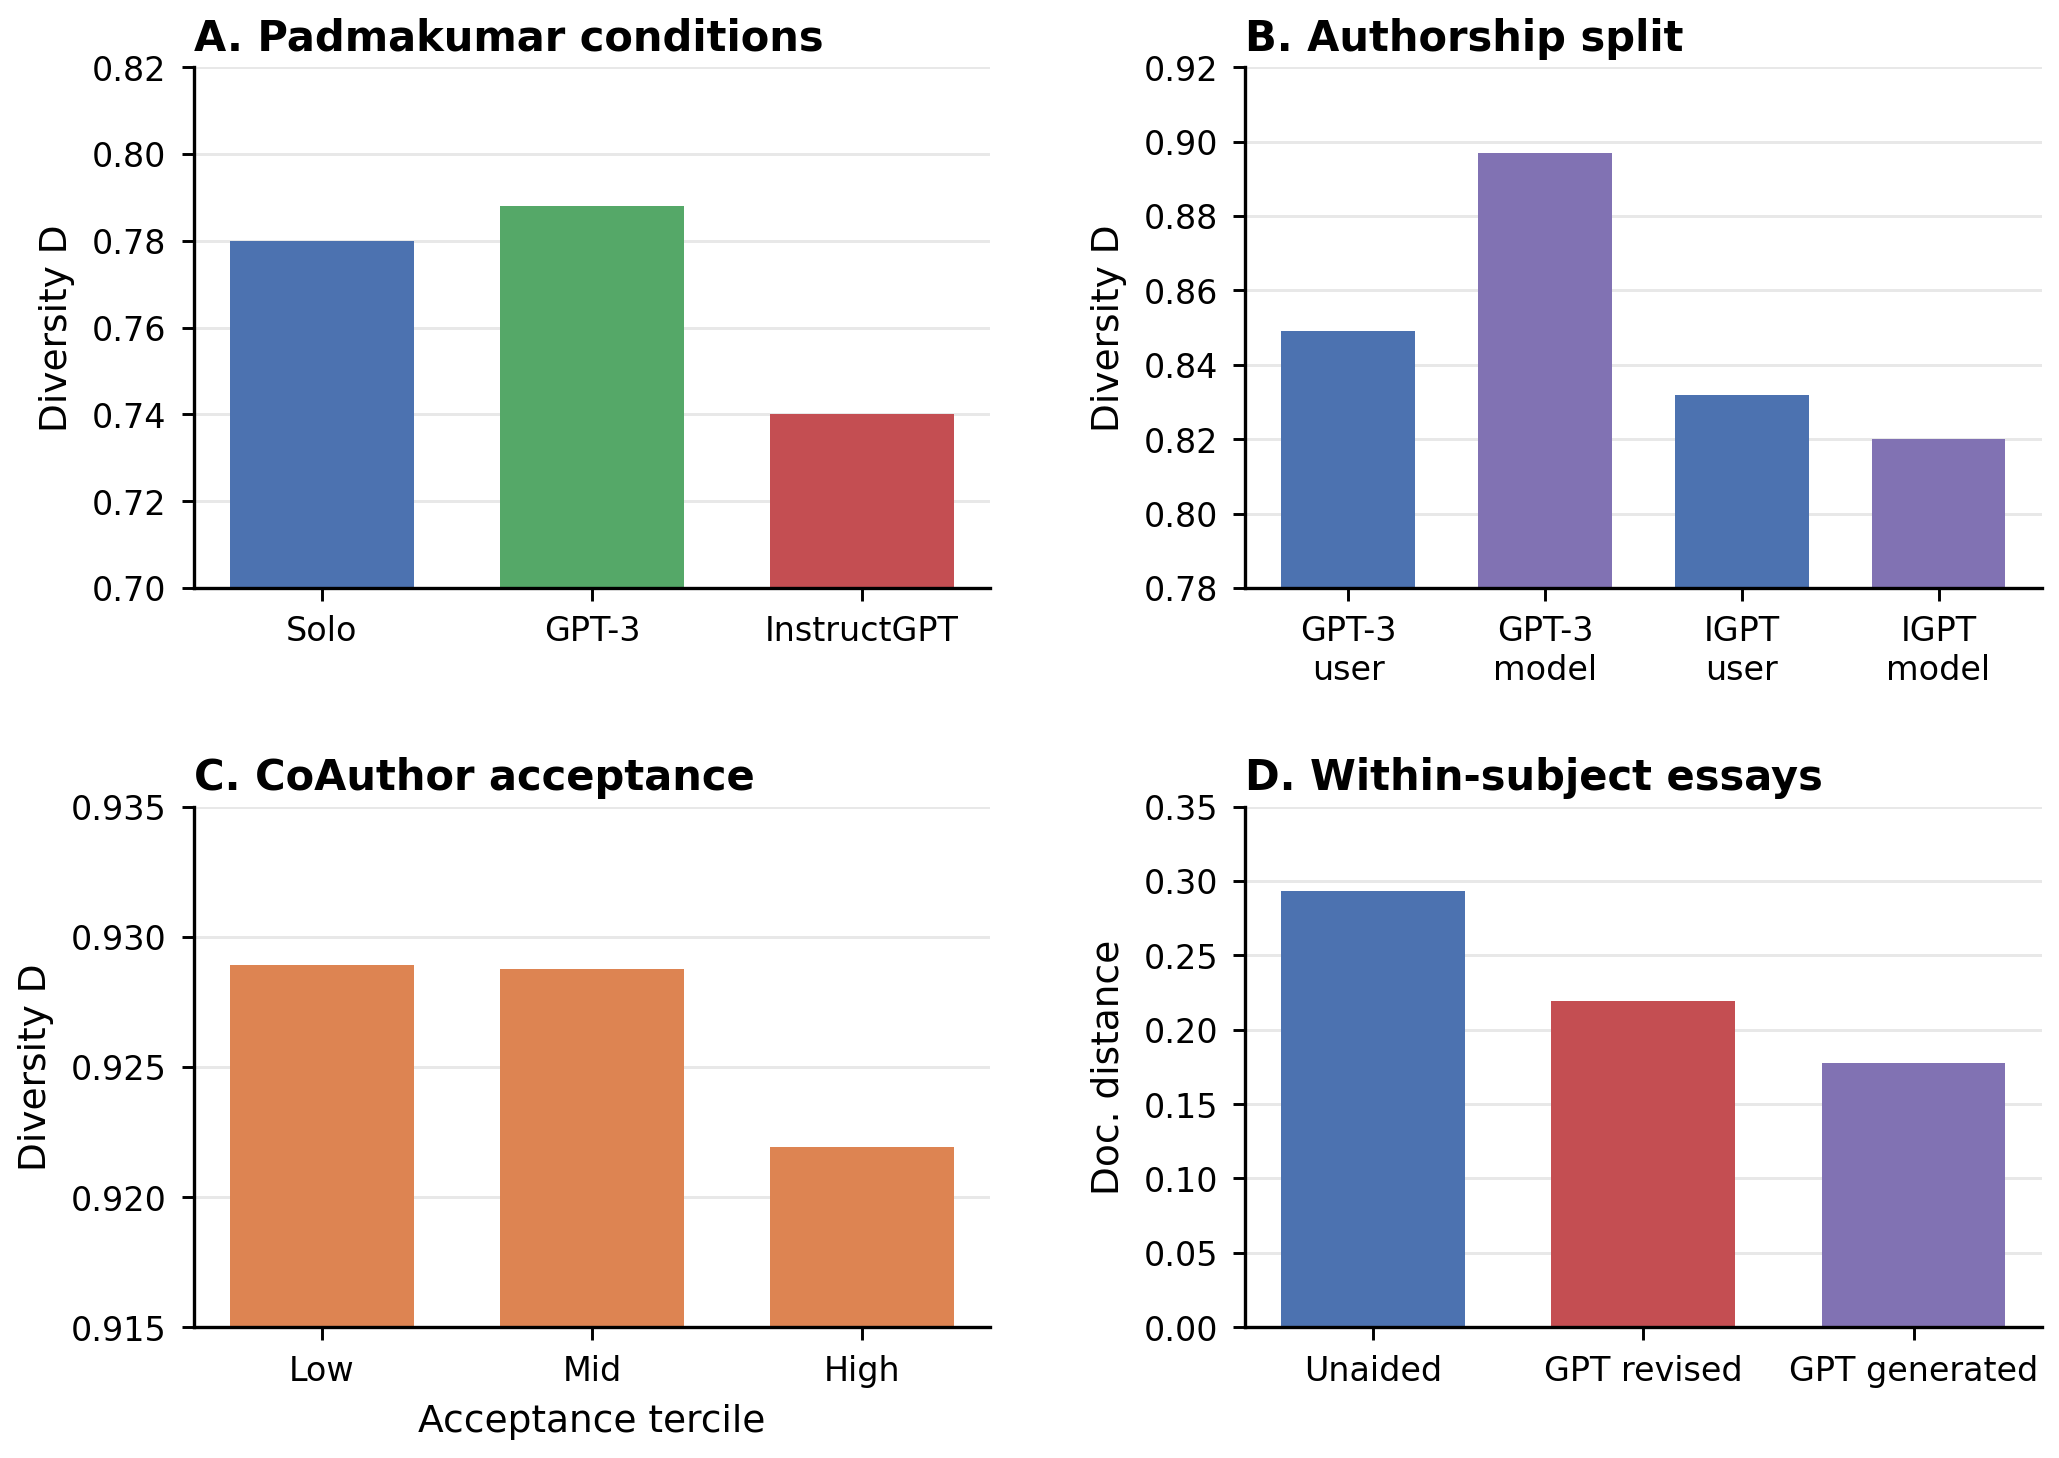
\includegraphics[width=\linewidth]{figures/fig_multicorpus.png}}

\section{Discussion}

The result worth keeping is precise and limited.
A shared feedback-tuned prior can pull co-written essays closer together~\citep{padmakumar2024diversity}.
Permutation tests and the GPT-3 contrast interval back that claim; the solo--InstructGPT bootstrap interval remains wide.
Base GPT-3 does not reproduce the drop, so homogenization is better explained by the prior people share than by help as such.

The larger cognitive-convergence package does not earn the same status in these public files.
CoAuthor lacks a clear acceptance-to-diversity dose curve~\citep{lee2022coauthor}.
Moon et al.\ show that the model itself is a narrow attractor, while observational word diversity does not fall after ChatGPT~\citep{moon2026disjunction}.
Text homogenization is not proof of offloading.
Debt remains a separate question wherever unaided controls are missing.

For evaluation practice, report three quantities apart: assisted quality, cross-person diversity under a shared tool, and tool-removed transfer.
A full conference paper would need a new controlled study; this note only ranks existing public evidence.

\section{Limitations}

Padmakumar spans ten topics, so topic-bootstrap intervals are wide; the solo versus InstructGPT CI includes zero even though the permutation test is significant.
Authorship compression under InstructGPT is directional but not tightly estimated.
CoAuthor dose analyses are correlational and lack solo writing.
Moon observational contrasts confound year with possible AI use.
Learning-companion arms have no no-AI control.
This note is a public-data reassessment, not a new human experiment.
Era-level Moon document-distance aggregates reuse the released OSF summary tables rather than a full from-scratch re-derivation of every embedding distance.

\section*{Ethics statement}
This work reanalyzes publicly released research corpora.
No new human subjects were recruited.
Upstream consent and licensing remain those of the original studies.

\section{Conclusion}

Public co-writing data support a limited claim: shared feedback-tuned priors can compress writing diversity.
They do not support a blanket claim that assistance homogenizes, and they do not establish unified cognitive convergence with proven transfer debt.
Keep the prior result. Drop the overclaim. Leave debt to designs that can actually test it.
This technical report is meant as a workshop-scale evidence map, not as a substitute for a new experiment.

\section*{Data and code}
Upstream corpora:
\begin{itemize}
  \item Padmakumar and He: \url{https://github.com/vishakhpk/hai-diversity}
  \item CoAuthor: \url{https://coauthor.stanford.edu}
  \item Moon et al.: \url{https://doi.org/10.17605/OSF.IO/YD94Z}
  \item Study companion: \url{https://doi.org/10.17605/OSF.IO/SWYTK}
\end{itemize}
Analysis code, paper tables, and figure scripts:\\
\url{https://github.com/baban9/shared-priors-homogenization}

\section*{Acknowledgments}
The author thanks the creators of the public corpora reanalyzed here.
This preprint reports an independent reanalysis; any errors are the author's.

\section*{Competing interests}
The author declares no competing interests.

\bibliographystyle{plainnat}
\bibliography{references}

\end{document}
